% time values for run2 and run3
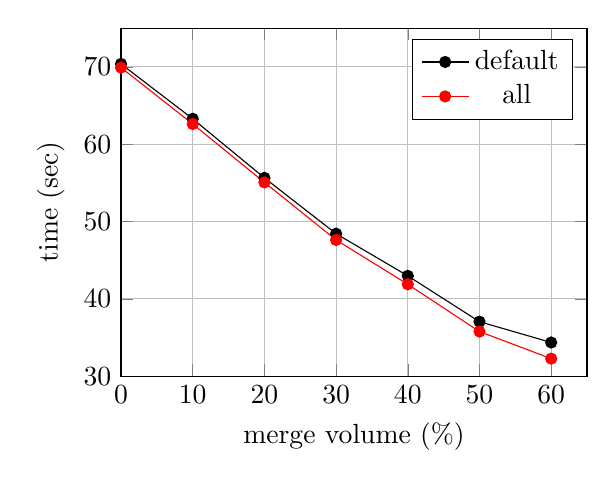
\begin{tikzpicture}
\begin{axis}[
    title={},
    height=6cm,
    width=7.5cm,
    xlabel={merge volume (\%)},
    ylabel={time (sec)},
    xmin=0, xmax=65,
    ymin=30, ymax=75,
    xtick={0,10,20,30,40,50,60},
    ytick={30,40,50,60,70},
    legend pos=north east,
    xmajorgrids=true,
    ymajorgrids=true,
]

\addplot[
    color=black,
    mark=*
    ]
    coordinates {
    (0,70.38)(10,63.28)(20,55.64)(30,48.42)(40,42.97)(50,37.04)(60,34.35)
    };
    
\addplot[
    color=red,
    mark=*
    ]
    coordinates {
    (0,69.91)(10,62.61)(20,55.06)(30,47.61)(40,41.88)(50,35.76)(60,32.26)
    };
    
\legend{default, all}
    
\end{axis}
\end{tikzpicture}